
%%%%%%%%%%%%%%%%%%%%%%%%%%%%%%%%%%%%%%%%%%%%%%%%%%%%%%%%%%%%%%%%%%%%%%%%%%%%%%
\section{Option 1: converter mounted on a moving arm} 
A configuration of the Mu2e detector with the pion degrader,
as shown in  Figure~\ref{figure:degrader_geometry_v3}, inserted in the beam has been simulated.

\begin{itemize}
\item 
  From \piplusenu\ studies: the pion degrader disk thickness of 4 mm Ti
  is close to optimal\cite{MU2E_48630_PIPLUSENU}.
\item
  4mm of Ti correspond to the total amount of material of $\sim 1.8 ~g/cm^2$,
  about twice the material of the stopping target.
\item
  to keep the thickness of the degrader disk below 1 cm, the degrader implemented
  out of two layers: $CH_2$ and Pb.
  \begin{itemize}
  \item 
    9mm CH2 + 1.0mm Pb: : $\rm 2.0  ~g/cm^2$   .. $\pi*15^2*(0.9*0.95 + 11.34): \simeq 2 ~g/cm^2$
  \item
    9mm CH2 + 0.8mm Pb: : $\rm 1.76 ~g/cm^2$
  \item
    the weight of the disk: \\
    CH2 disk R=14 cm, weight        : $0.90*0.95*\pi*14^2 ~= 526$ gr \\
    Pb  foil R=10cm thickness 0.8mm : $0.08*11.34*\pi*10^2 = 285$ gr \\
    total                           : 811 gr
  \end{itemize}
 \item 
   As simulated, the gold converter ring has the outer radius $R_{out}$ = 250mm.
   The value of $R_{in}$ is defined by the converter thickness.
   The converter is slightly offset downstream with respect to the $CH_2$ disk,
   so the \eplus\ and \eminus\ produced in the converter do not cross it multiple times.

\end{itemize}

For small, of the order of few cm, widths of the converter ring,
the acceptance is proportional to the width.
So making the width, for example, 3cm instead of 1 cm wide would increase
the acceptance by a factor close to x3. However, the space between the OPA
and the TS available
for the degrader installation is limited, about 5 cm along the Z axis, 
and that limits the maximal width of the converter ring. Also, a large radius
of the converter ring, R = 25-30 cm, could start limiting the movement of the
degrader arm.

A potentially more attractive alternative could be to have the converter placed
on a thin carbon foam ring and supported inside the OPA. In this case,
the width of the foil could be increased without introducing the space conflicts.
Having the converter supported by the OPA would also simplify increasing
the converter radius, should that become necessary.
%
This option is discussed in Section~\ref{section:geometry_v4}


%%%%%%%%%%%%%%%%%%%%%%%%%%%%%%%%%%%%%%%%%%%%%%%%%%%%%%%%%%%%%%%%%%%%%%%%%%%%%%
\newpage
\subsection{Stopped negative pions}

Simulation of the negative pion beam follows the standard Mu2e two-stage model.
Stage 2 produces three separate datasets of pions stops in the CH2, Pb, and the ST.
The scheme allows to re-simulate the pion stop datasets for different degrader geometries
w/o repeating the first simulation stage, which significantly more time consuming.
To improve the simulation efficiency, pion decays are disabled and calculated by Geant4
pion survival probabilities are used as event weights in the normalization procedure.

Distributions of momentum and time of pions stopped in it CH2, Pb foil, and the
stopping target are shown in Figure \ref{figure:stopped_pim_mom_time}.
Each histogram entry has a weight of the respective pion survival probability.

\begin{figure}[H]
  \begin{tikzpicture}
    \node[anchor=south west,inner sep=0] at (0,0.) {
      % \node[shift={(0 cm,0.cm)},inner sep=0,rotate={90}] at (0,0) {}
      % \makebox[\textwidth][c] {
        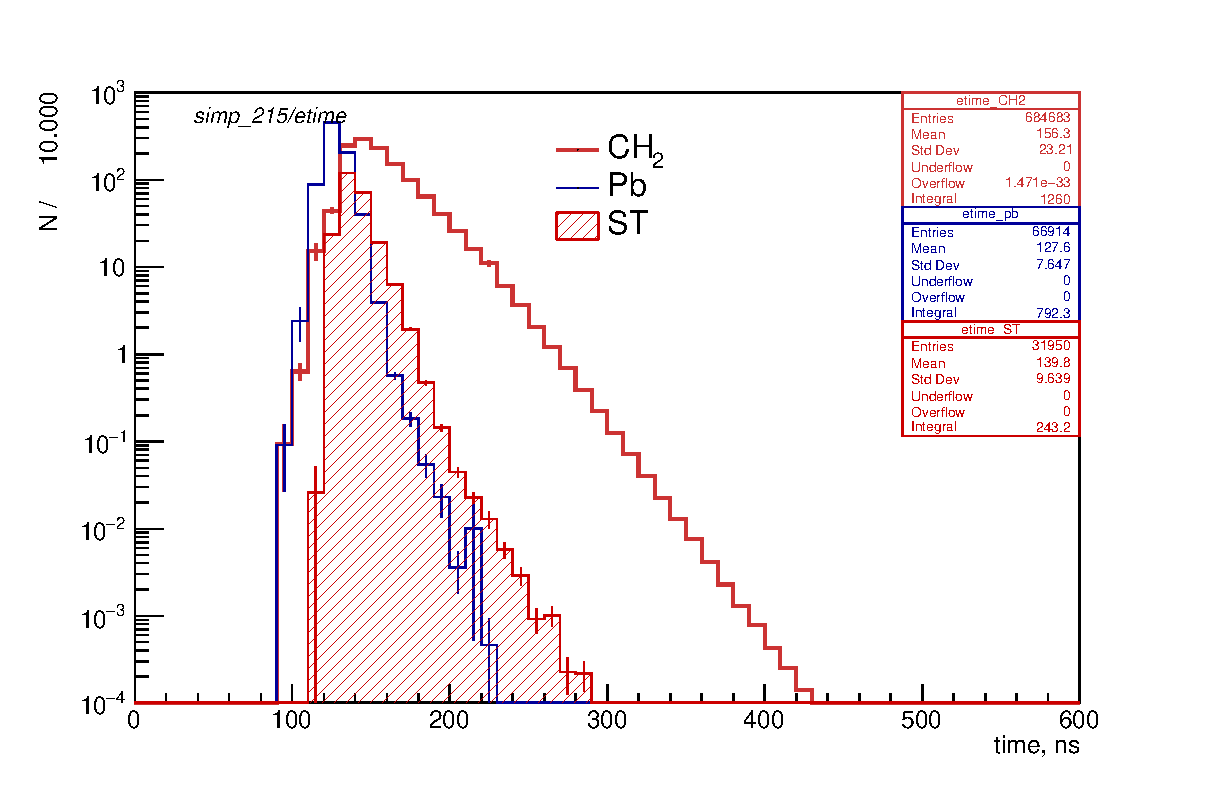
\includegraphics[width=0.5\textwidth]{pdf/figure_00021}
      % }
    };
    \node[anchor=south west,inner sep=0] at (10,0.) {
      % \node[shift={(0 cm,0.cm)},inner sep=0,rotate={90}] at (0,0) {}
      % \makebox[\textwidth][c] {
        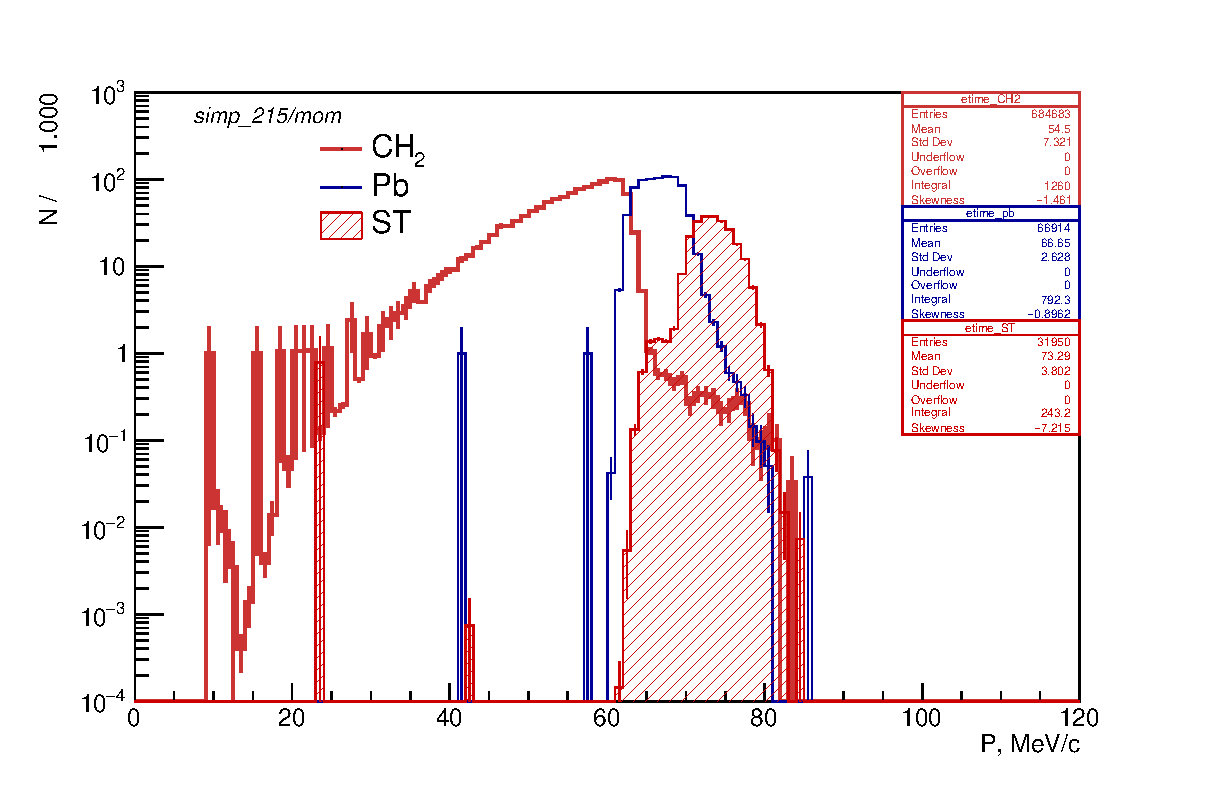
\includegraphics[width=0.5\textwidth]{pdf/figure_00022}
      % }
    };
    % \node [text width=8cm, scale=1.0] at (14.5,0.5) {$\mu_B$, expected background mean};
    % \node [text width=8cm, scale=1.0, rotate={90}] at (1.5,7.5) { $S_{D}$, ``discovery'' signal strength  };
  \end{tikzpicture}
  \caption{
    \label{figure:stopped_pim_mom_time}
    Stopped pions: distributions of momentum and time
  }
\end{figure}

It is worth noting that stopped in the $CH_2$ are the slowest pions.
Therefore, selecting events with the pion stop time above certain threshold,
i.e. $\sim 200$ ns, suppresses contributions of the stopping target
and the Pb foil to any measurement.
%
$T_0 = 200$ ns is also approximately the time where the instantaneous beam flash 
hit rate gets reduced down to the acceptable level, allowing the measurements.
For the DAQ operations, that means that the digitization start time should
be lowered to $\sim 250$ ns, which, at a reduced proton beam intensity,
looks quite realistic.

Another correlation to note is the correlation between the pion momentum
on exit from the TS momentum and the vertical coordinate of the pion stop.
Figure ~\ref{figure:y_vs_p_deg} shows this correlation for pions stopped
in the $CH_2$ and Pb parts of the degrader.
%
The Y distribution of pion stops in the Pb foil is offset down by several centimeters.
The lower cut-off at R=100 mm is determined by the by the simulated radius of the Pb foil.

\begin{figure}[H]
  \begin{tikzpicture}
    \node[anchor=south west,inner sep=0] at (0,0.) {
      % \node[shift={(0 cm,0.cm)},inner sep=0,rotate={90}] at (0,0) {}
      %\makebox[\textwidth][c] {
        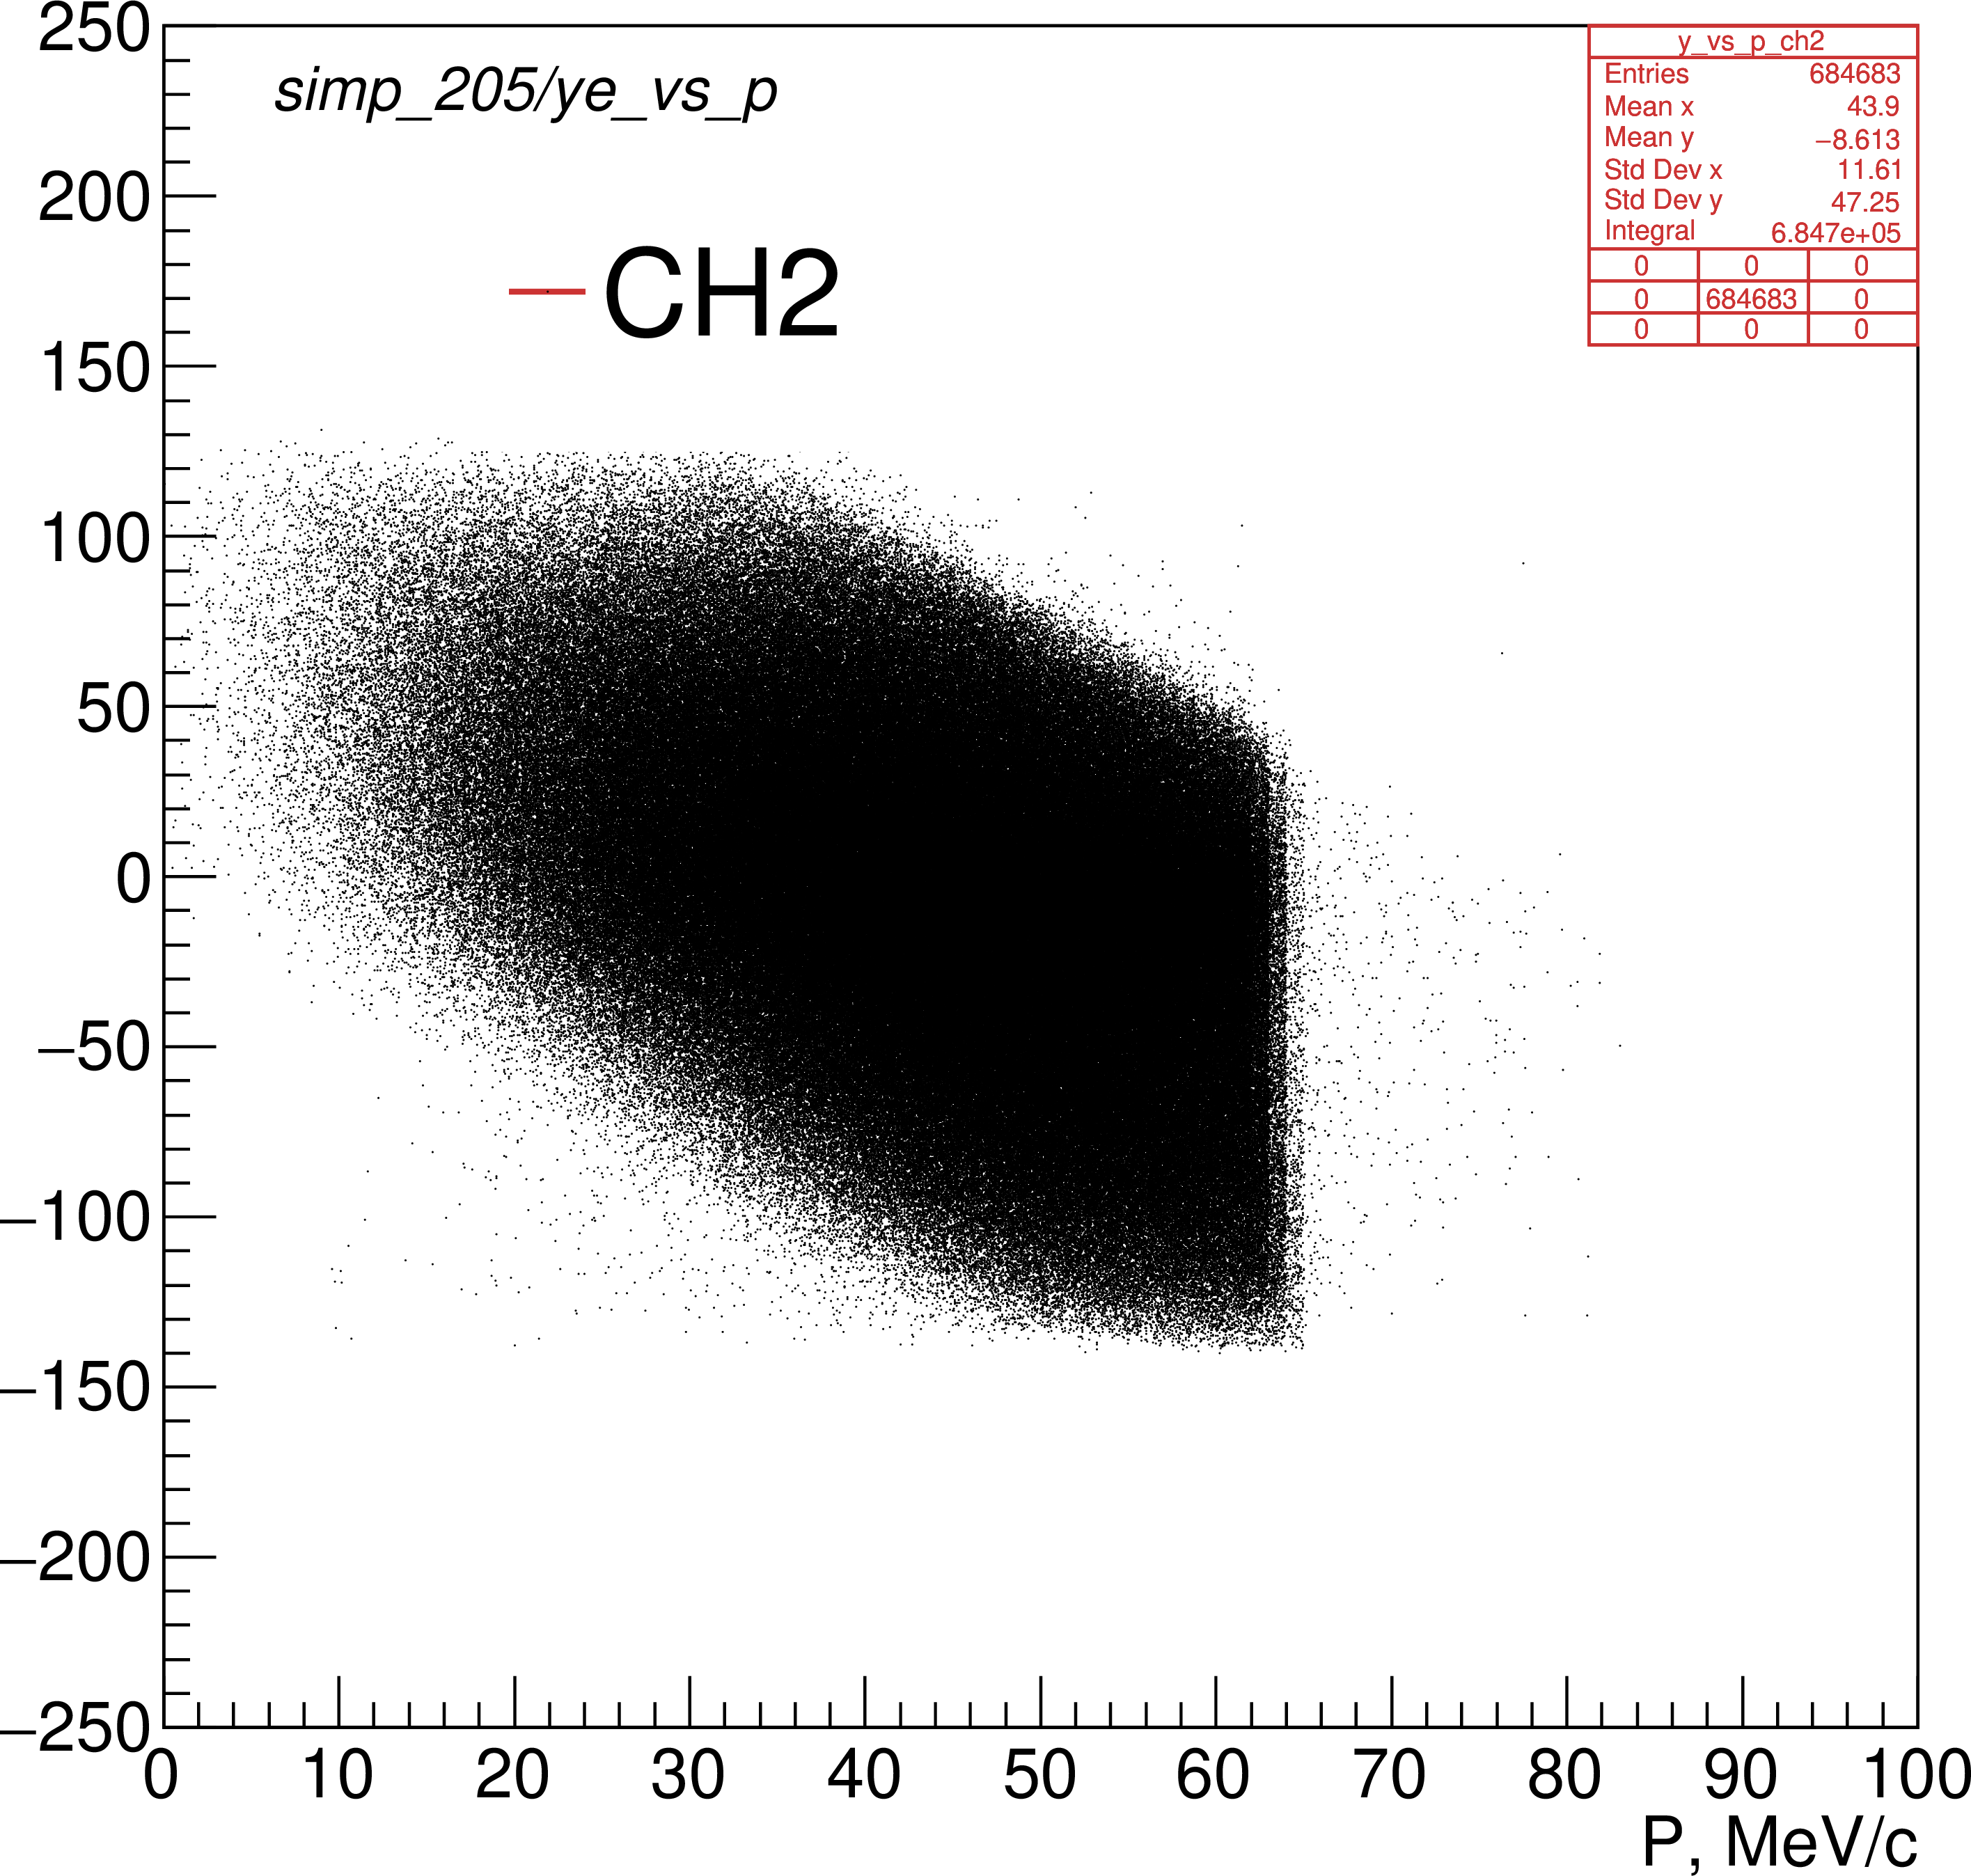
\includegraphics[width=0.5\textwidth]{png/figure_00036}
      %}
    };
    \node[anchor=south west,inner sep=0] at (10.,0.) {
      % \node[shift={(0 cm,0.cm)},inner sep=0,rotate={90}] at (0,0) {}
      % \makebox[\textwidth][c] {
      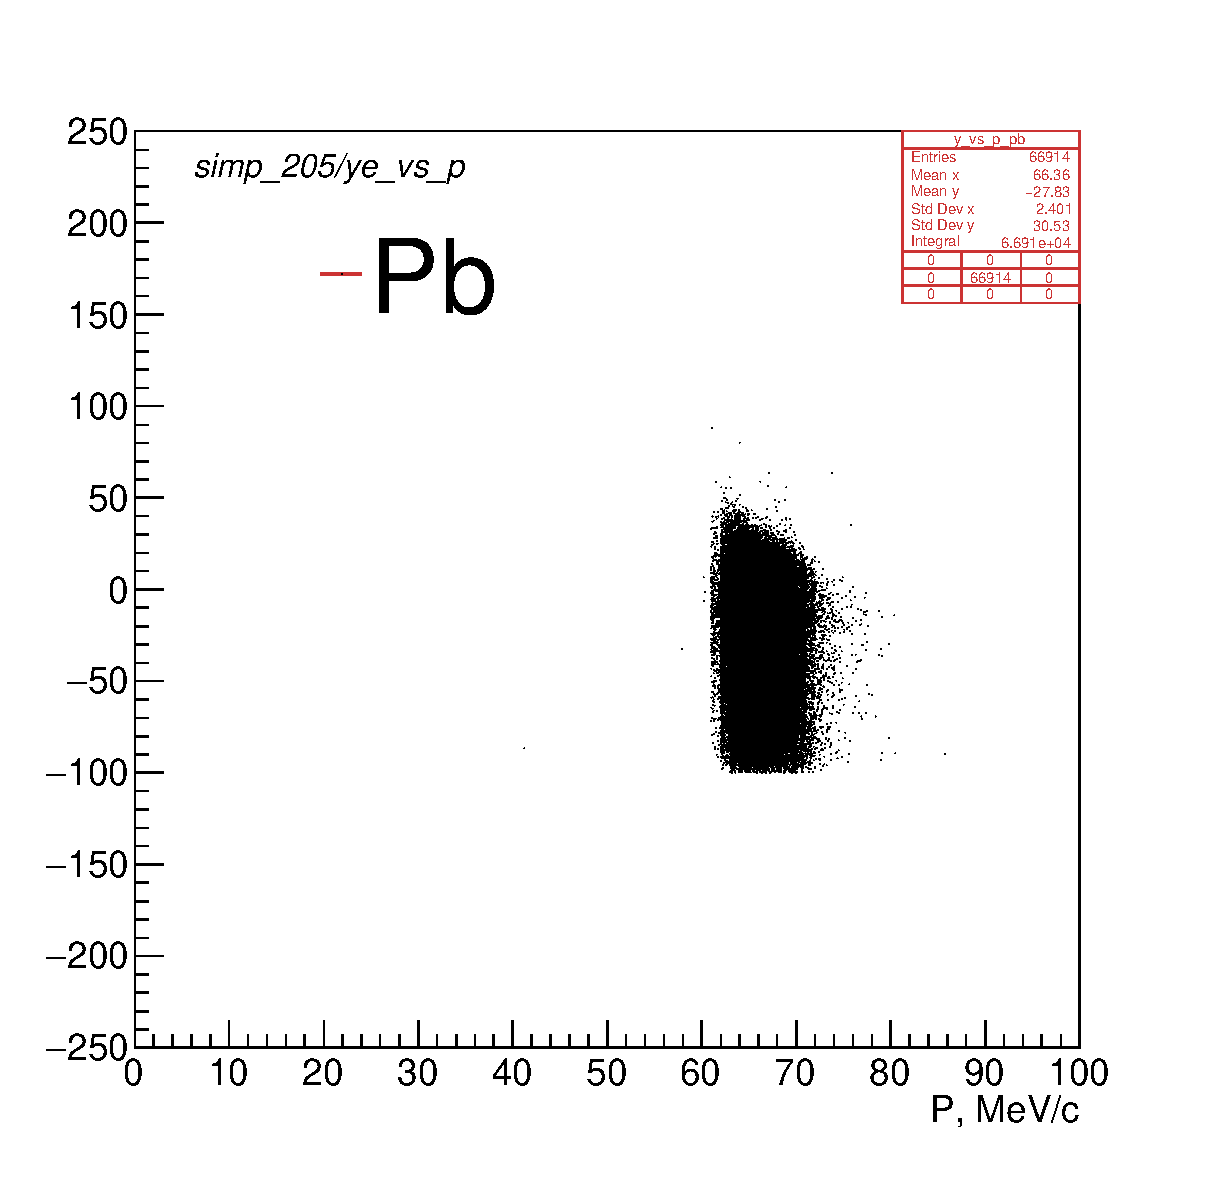
\includegraphics[width=0.5\textwidth]{png/figure_00037}
      %} 
    };
    % \node [text width=8cm, scale=1.0] at (14.5,0.5) {$\mu_B$, expected background mean};
    % \node [text width=8cm, scale=1.0, rotate={90}] at (1.5,7.5) { $S_{D}$, ``discovery'' signal strength  };
  \end{tikzpicture}
  \caption{
    \label{figure:y_vs_p_deg}
    Y(stop):P at DS entrance for $\pi^-$'s stopped in the $CH_2$ and Pb parts of the simulated degrader
  }
\end{figure}

Y:X distributions of the pion stops in the $CH_2$ disk, Pb foil and the ST are shown in Figure ~\ref{figure:y_vs_x_st}.
They reflect the correlation between the mean Y of the particle trajectory and the particle momentum.

\begin{figure}[H]
  \begin{tikzpicture}
    \node[anchor=south west,inner sep=0] at (0,0.) {
      % \node[shift={(0 cm,0.cm)},inner sep=0,rotate={90}] at (0,0) {}
      %\makebox[\textwidth][c] {
        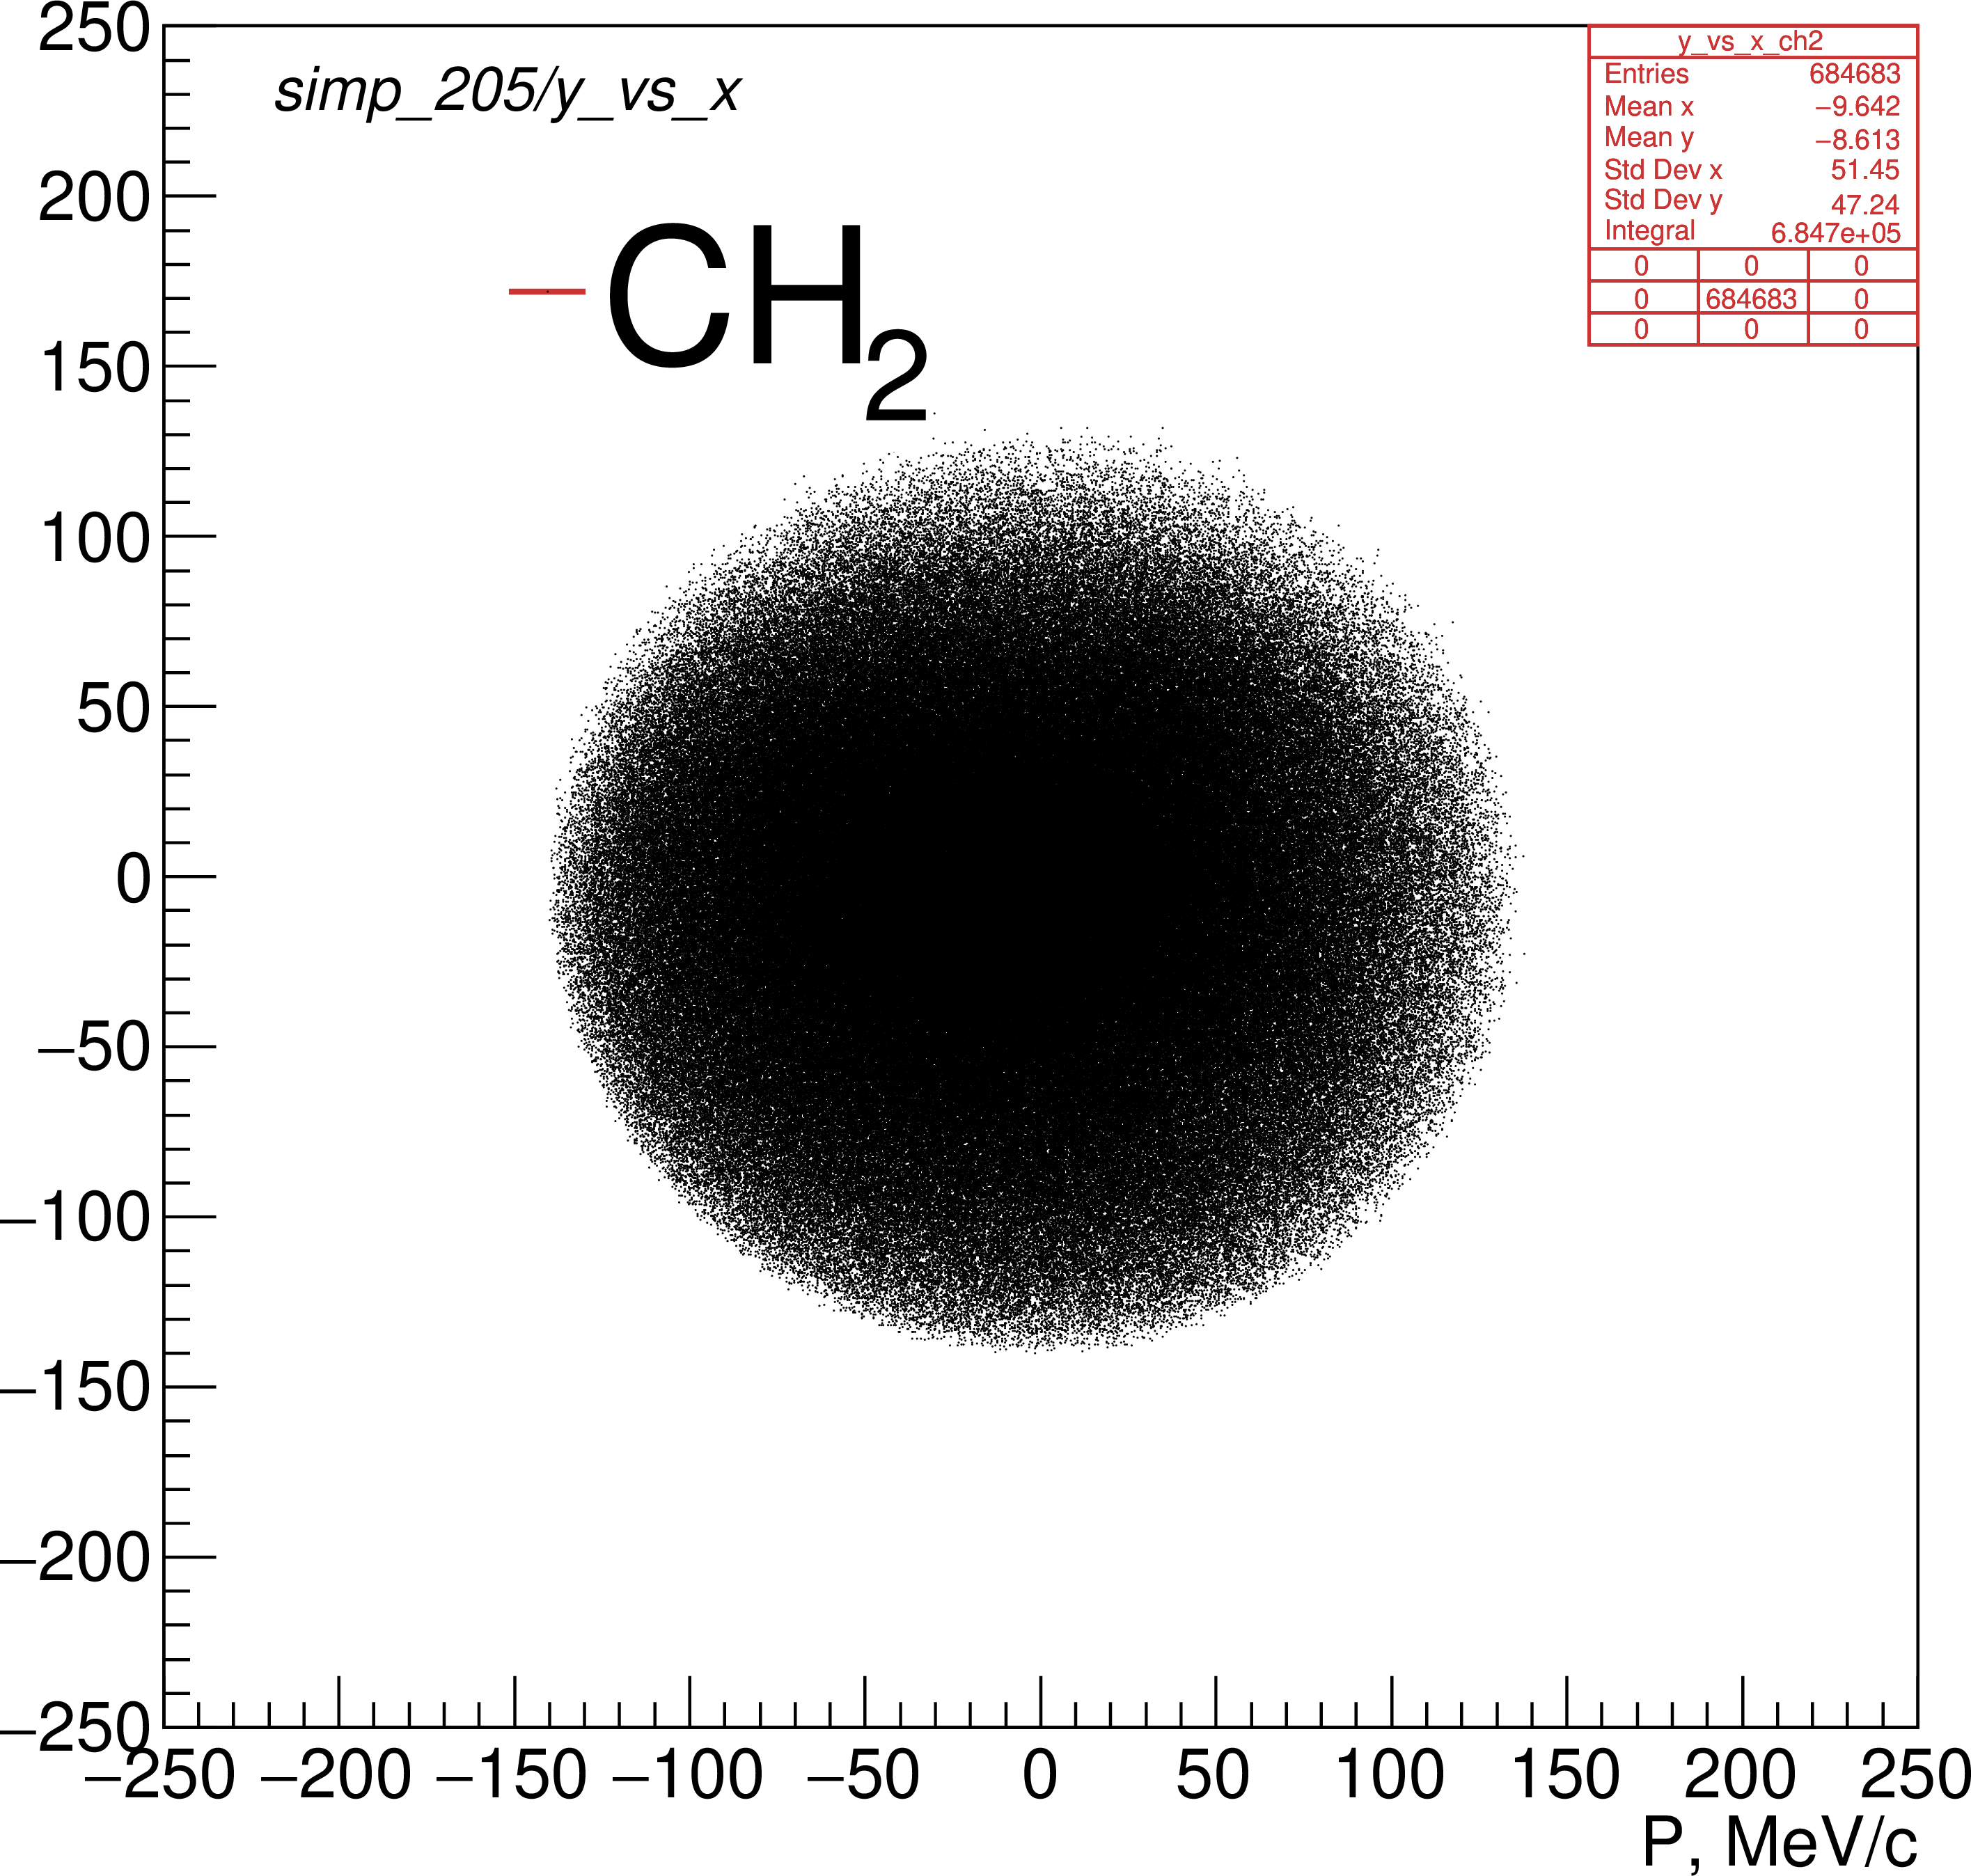
\includegraphics[width=0.5\textwidth]{png/figure_00034}
      %}
    };
    \node[anchor=south west,inner sep=0] at (10.,0.) {
      % \node[shift={(0 cm,0.cm)},inner sep=0,rotate={90}] at (0,0) {}
      %\makebox[\textwidth][c] {
        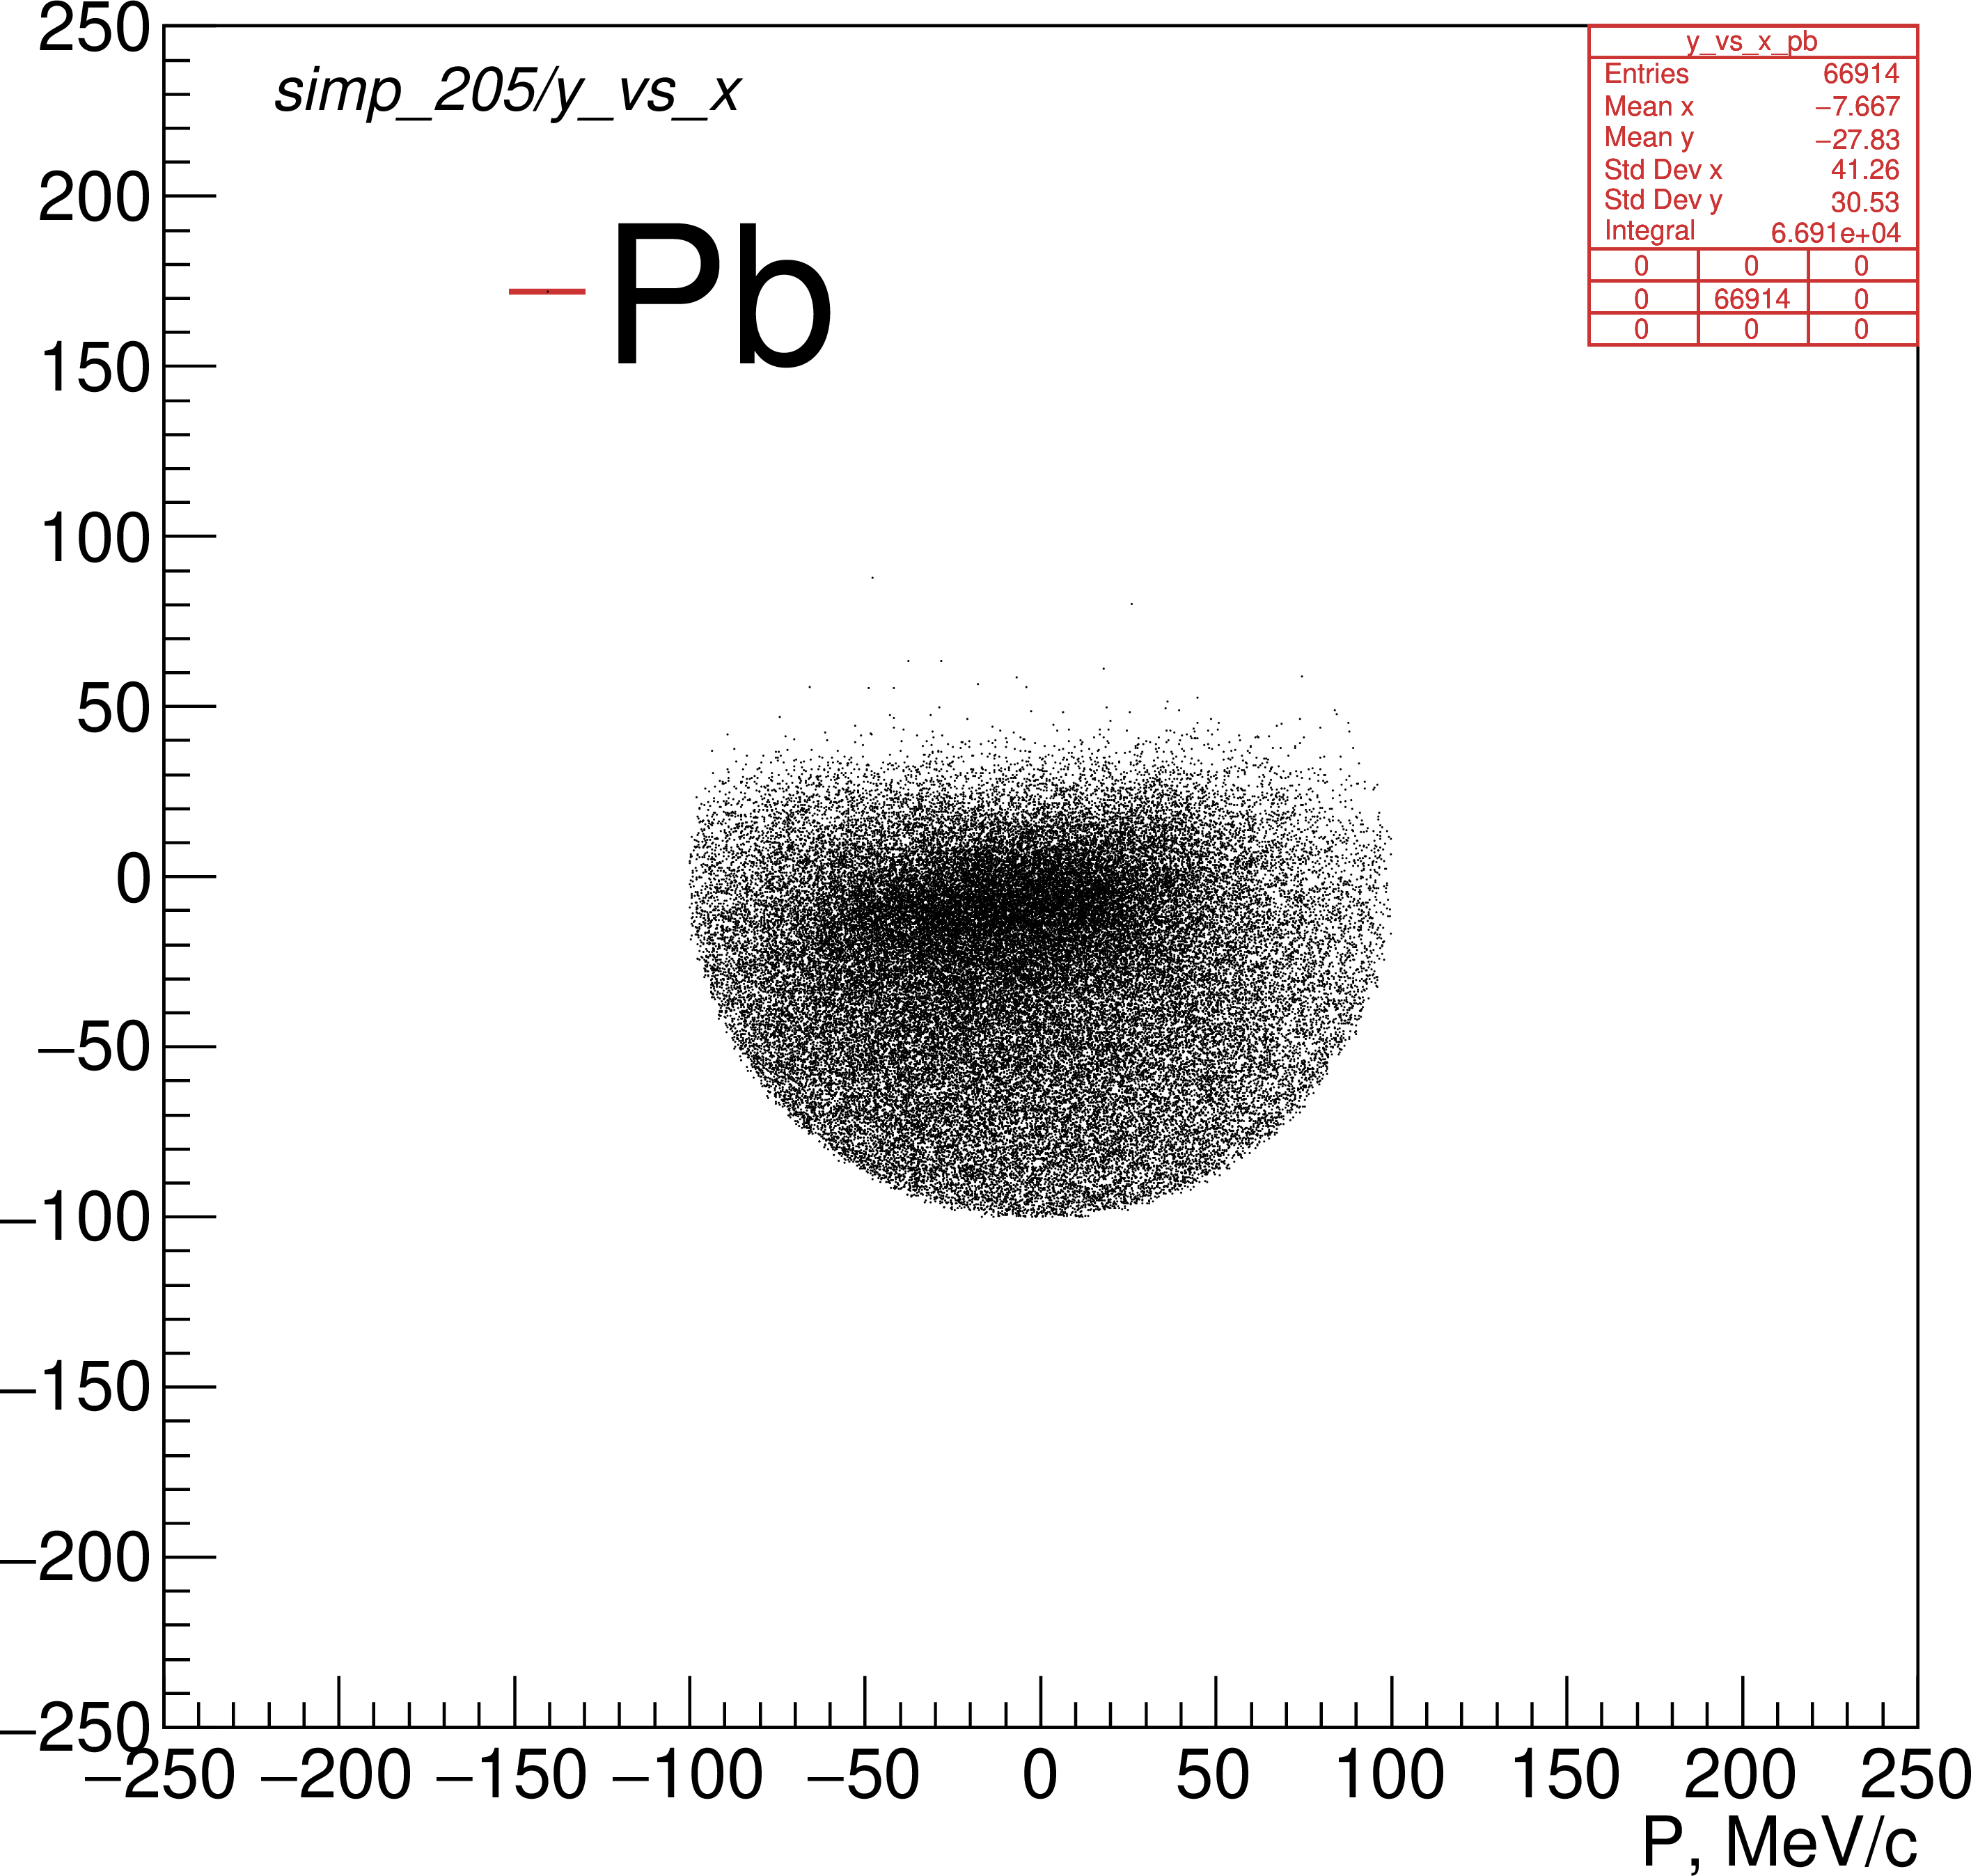
\includegraphics[width=0.5\textwidth]{png/figure_00035}
      %}
    };
    \node[anchor=south west,inner sep=0] at (0,-10.) {
      % \node[shift={(0 cm,0.cm)},inner sep=0,rotate={90}] at (0,0) {}
      % \makebox[\textwidth][c] {
        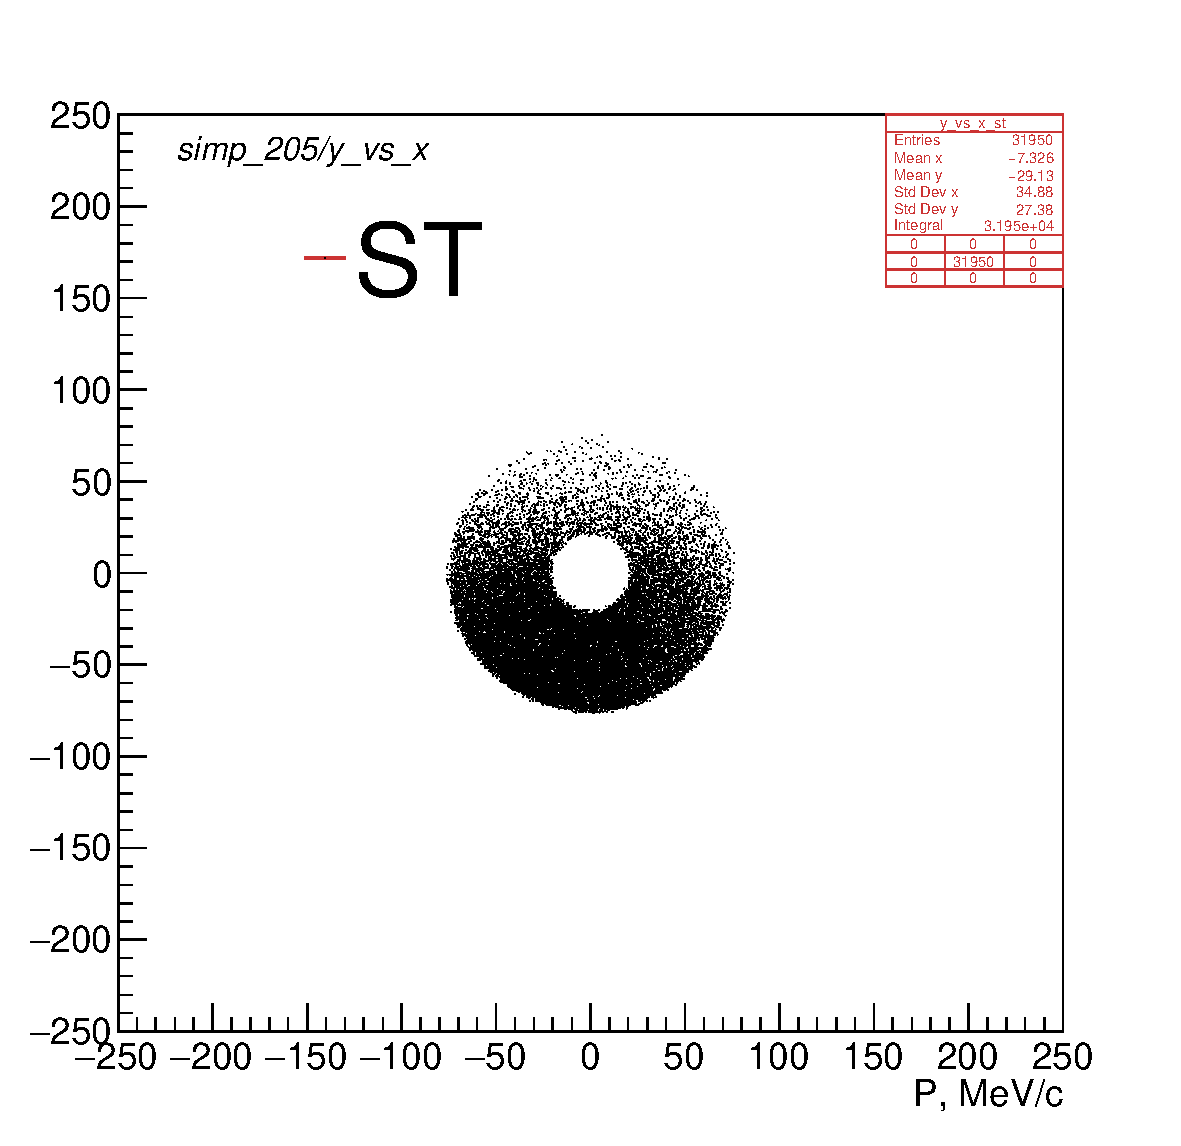
\includegraphics[width=0.5\textwidth]{png/figure_00031}
      % }
    };
    % \node [text width=8cm, scale=1.0] at (14.5,0.5) {$\mu_B$, expected background mean};
    % \node [text width=8cm, scale=1.0, rotate={90}] at (1.5,7.5) { $S_{D}$, ``discovery'' signal strength  };
  \end{tikzpicture}
  \caption{
    \label{figure:y_vs_x_st}
    Y(stop):X(stop) for pions stopped in the CH2, Pb, and ST
  }
\end{figure}

%%%%%%%%%%%%%%%%%%%%%%%%%%%%%%%%%%%%%%%%%%%%%%%%%%%%%%%%%%%%%%%%%%%%%%%%%%%%%%
\subsection{Reconstruction of the photon energy}

As photon is massless, in the production vertex, an electron and a positron
from $\gamma \to e^+e^-$ conversion have their momenta parallel to each other.
In that point, the photon energy can be approximated as
\begin{equation} \label{eq:egamma}
  E_\gamma = P(e^+) + P(e^-) 
\end{equation}
               
XY views of two typical events are presented in Figure~\ref{figure:rpc07b0s51r0100_xy_view},
Despite the fact that $e^+e^-$ pairs are produced several meters upstream of the tracker,
the multiple scattering is sufficiently small, and the \eplus\ and \eminus\ trajectories
in the tracker look like two tangent circles. Because of that, an approximation of Eq.{\ref{eq:egamma}}
should hold.

\begin{figure}[H]
  \begin{tikzpicture}
    \node[anchor=south west,inner sep=0] at (0,0.) {
      % \node[shift={(0 cm,0.cm)},inner sep=0,rotate={90}] at (0,0) {}
      \makebox[\textwidth][c] {
        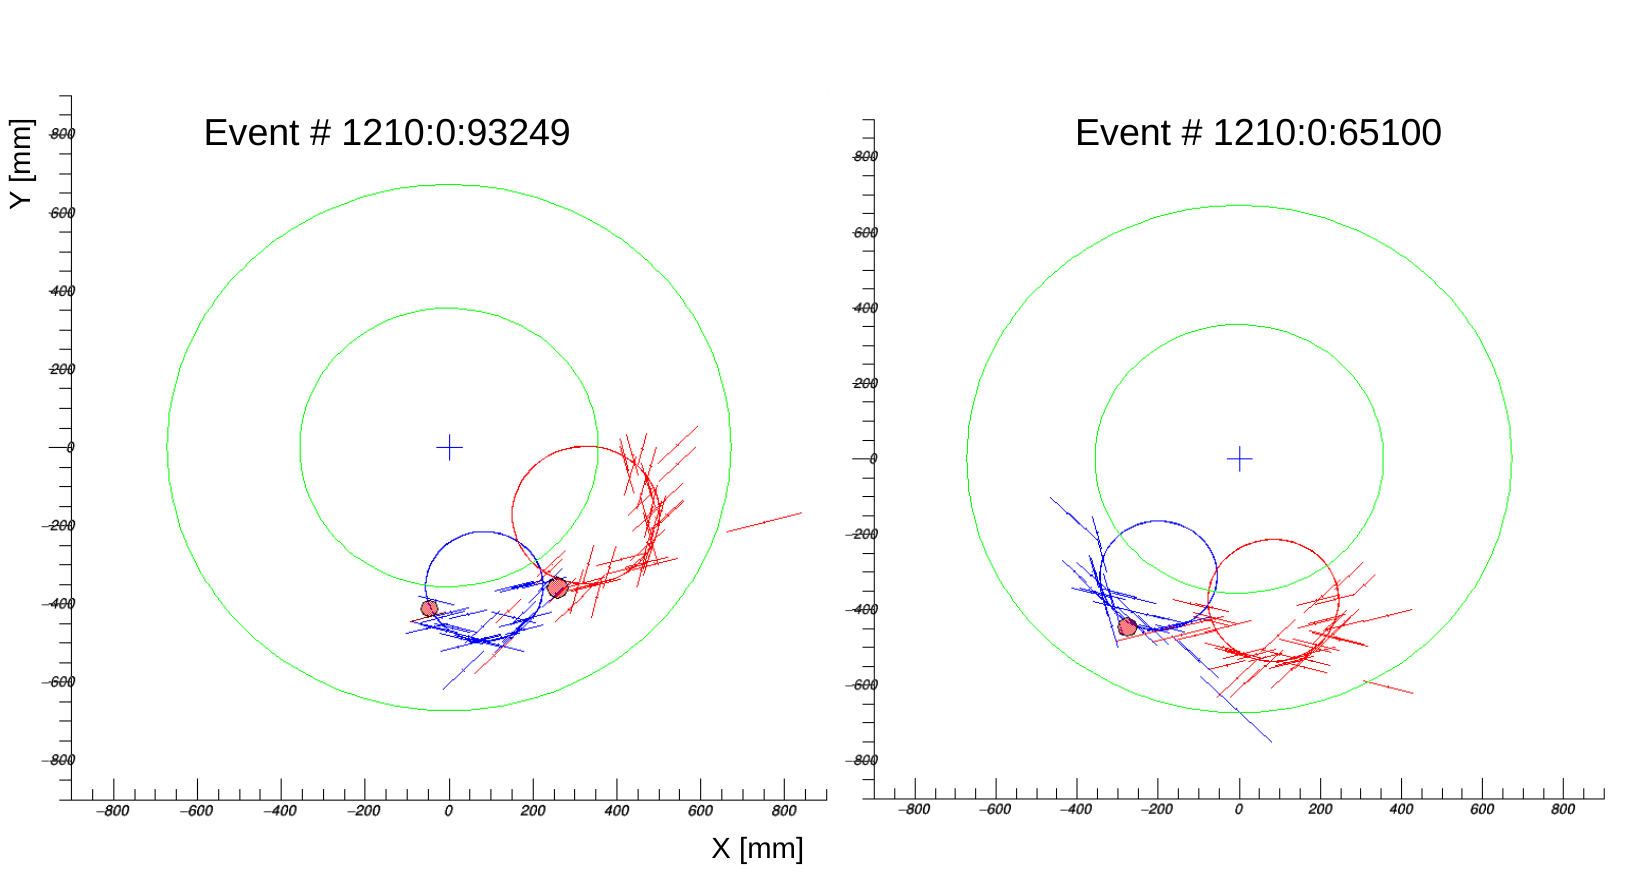
\includegraphics[width=0.9\textwidth]{png/rpc07b0s51r0100_event_display_xy_reconstructed}
      }
    };
    % \node [text width=8cm, scale=1.0] at (14.5,0.5) {$\mu_B$, expected background mean};
    % \node [text width=8cm, scale=1.0, rotate={90}] at (1.5,7.5) { $S_{D}$, ``discovery'' signal strength  };
  \end{tikzpicture}
  \caption{
    \label{figure:rpc07b0s51r0100_xy_view}
    XY tracker view of $\gamma \to e^+e^-$ events
  }
\end{figure}

%%%%%%%%%%%%%%%%%%%%%%%%%%%%%%%%%%%%%%%%%%%%%%%%%%%%%%%%%%%%%%%%%%%%%%%%%%%%%%
\subsection{Choice of the converter thickness}

The converter is simulated as a thin gold foil. To choose the optimal thickness ,
we considered three different options:
\begin{enumerate}
\item 
  1 mm-thick foil, 
\item
  200 um-thick foil, 
\item
 and 100 um -thick foil.
\end{enumerate}

Shown in Figure~\ref{figure:sum_mom_vd13}(left) are the distributions of $E_{gamma}^{VD13} = P(e^+)^{VD13} + P(e^-)^{VD13}$,
the scalar sum of MC momenta of an electron and a positron from a photon conversion
plotted for events with

\begin{itemize}
\item
  each of \eplus\ and \eminus\ producing N>=20 straw hits in the tracker;
\item
  minimal, out of the two, particle momentum P > 30 MeV/c at VD13 
\end{itemize}

\begin{figure}[H]
  \begin{tikzpicture}
    \node[anchor=south west,inner sep=0] at (0,0.) {
      % \node[shift={(0 cm,0.cm)},inner sep=0,rotate={90}] at (0,0) {}
      % \makebox[\textwidth][c] {
        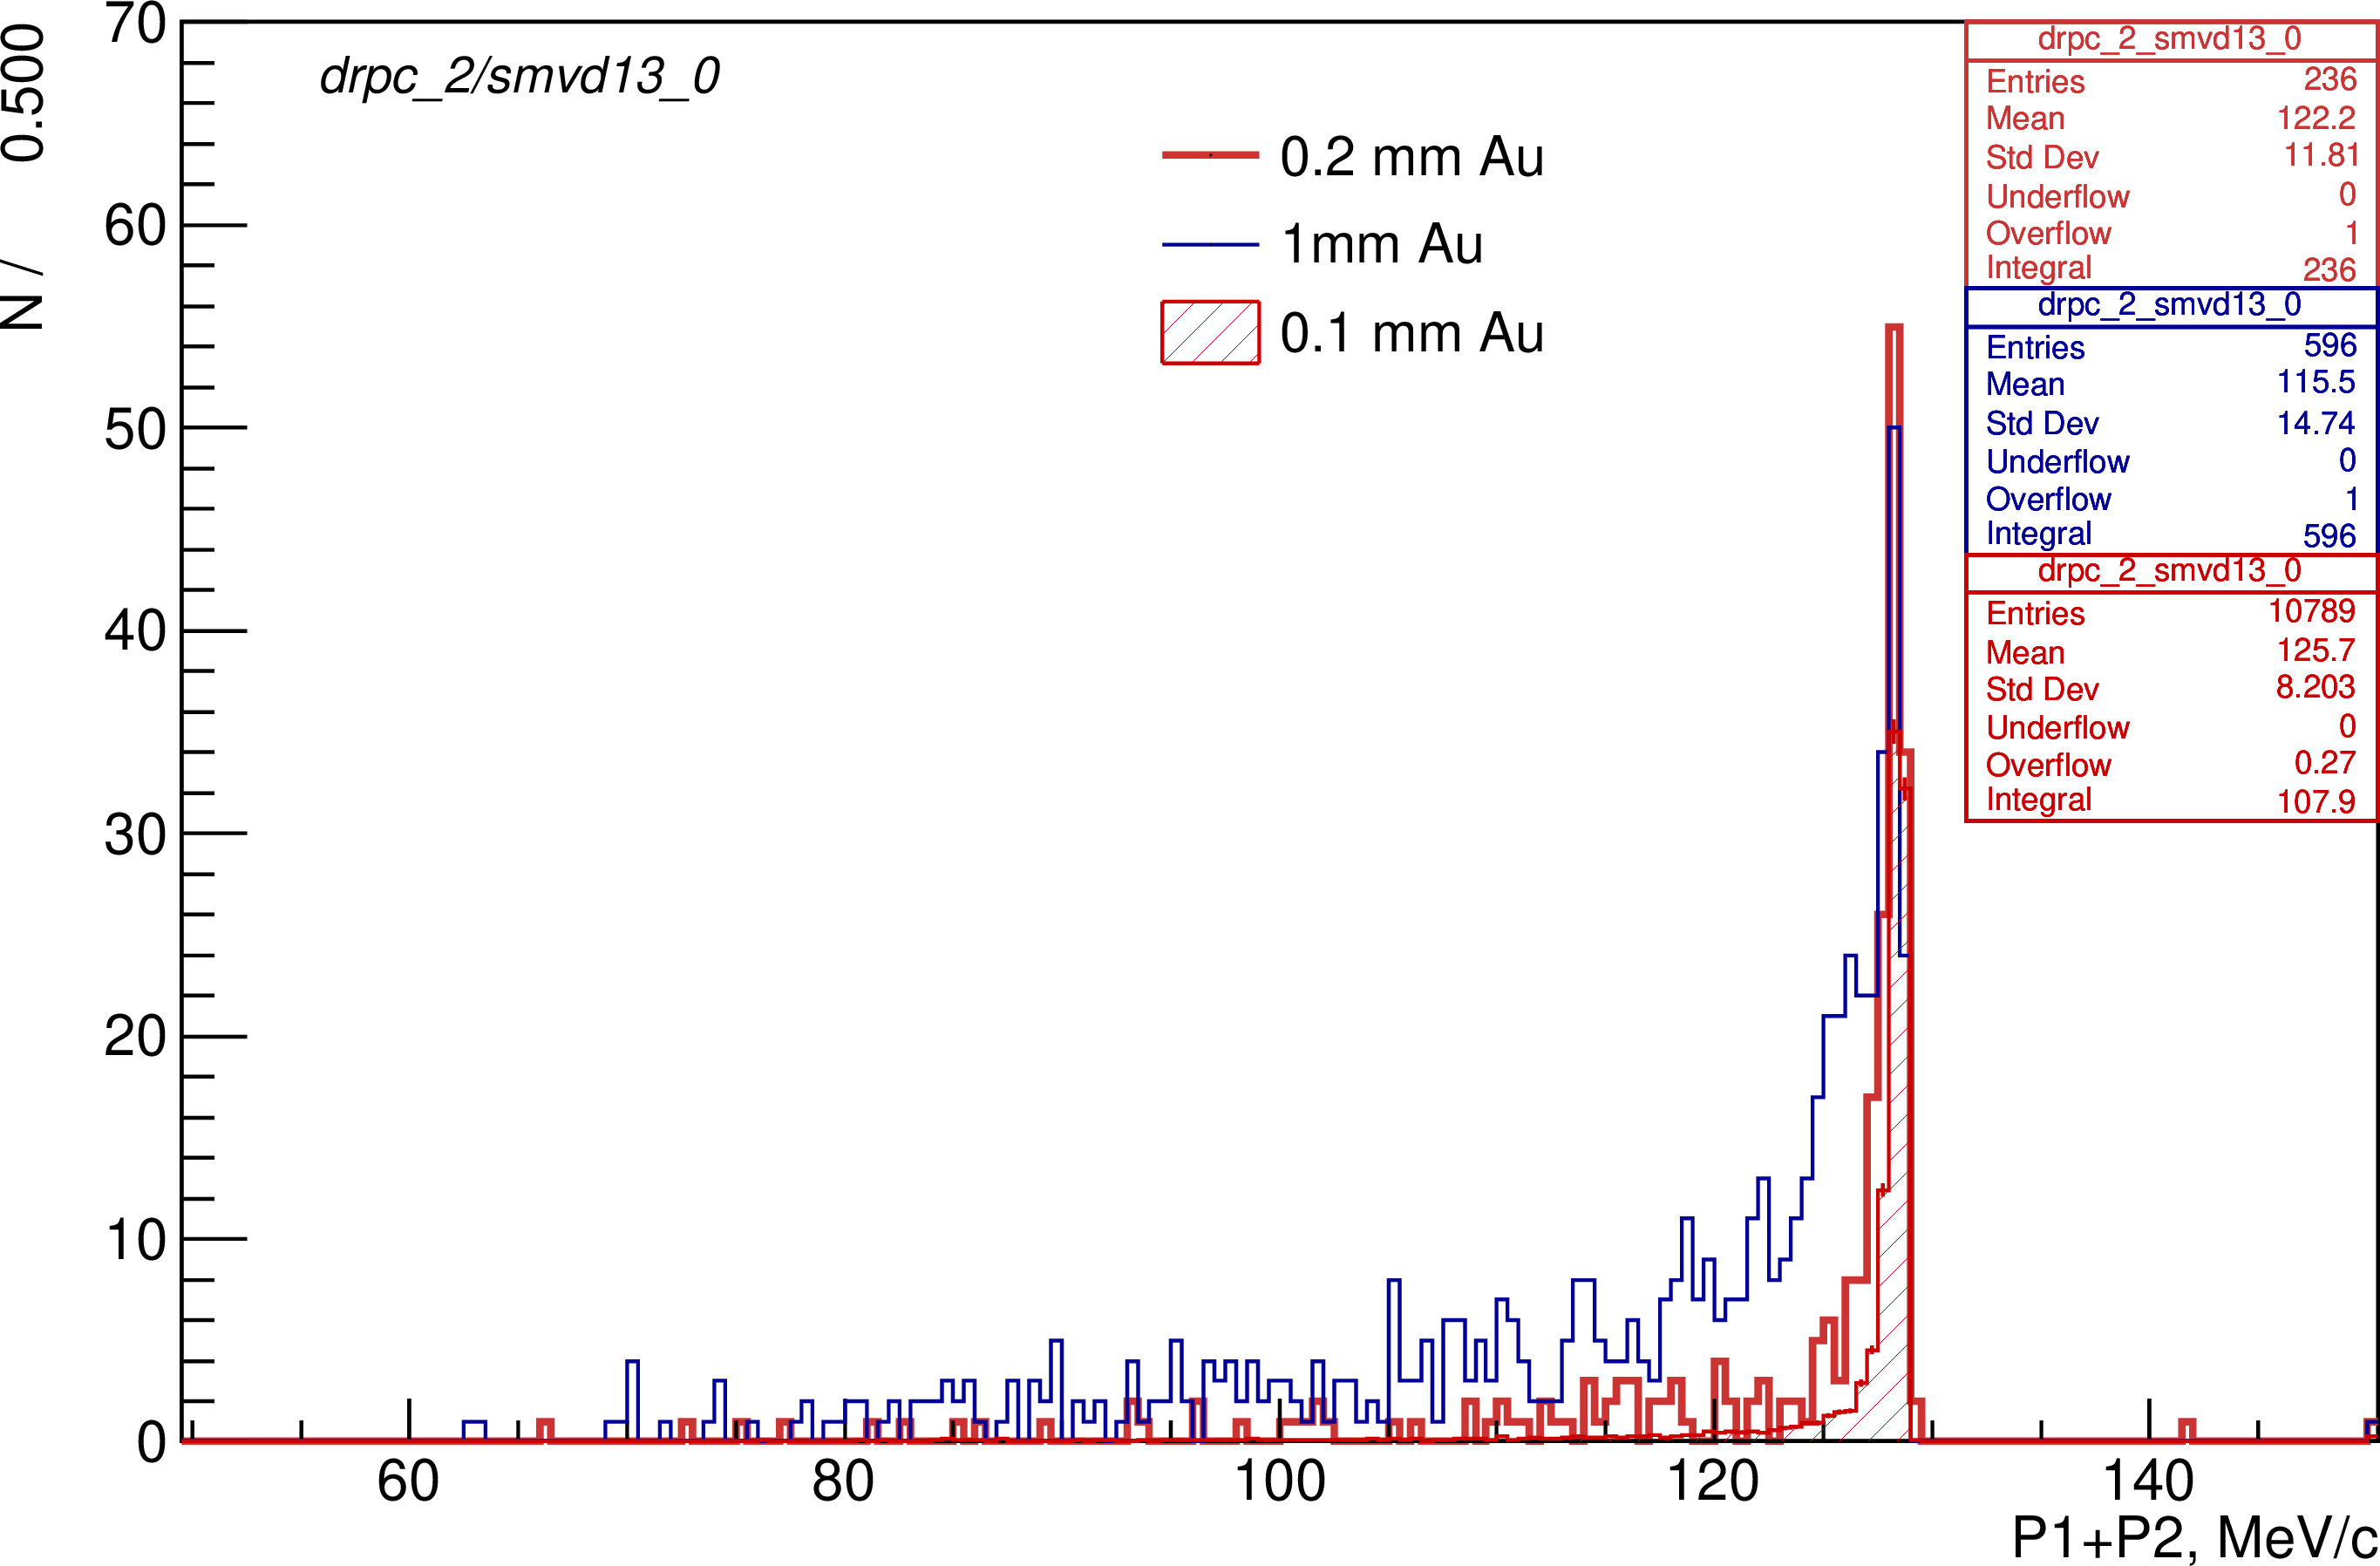
\includegraphics[width=0.54\textwidth]{pdf/figure_00013}
      % }
    };
    \node[anchor=south west,inner sep=0] at (10,0.) {
      % \node[shift={(0 cm,0.cm)},inner sep=0,rotate={90}] at (0,0) {}
      % \makebox[\textwidth][c] {
        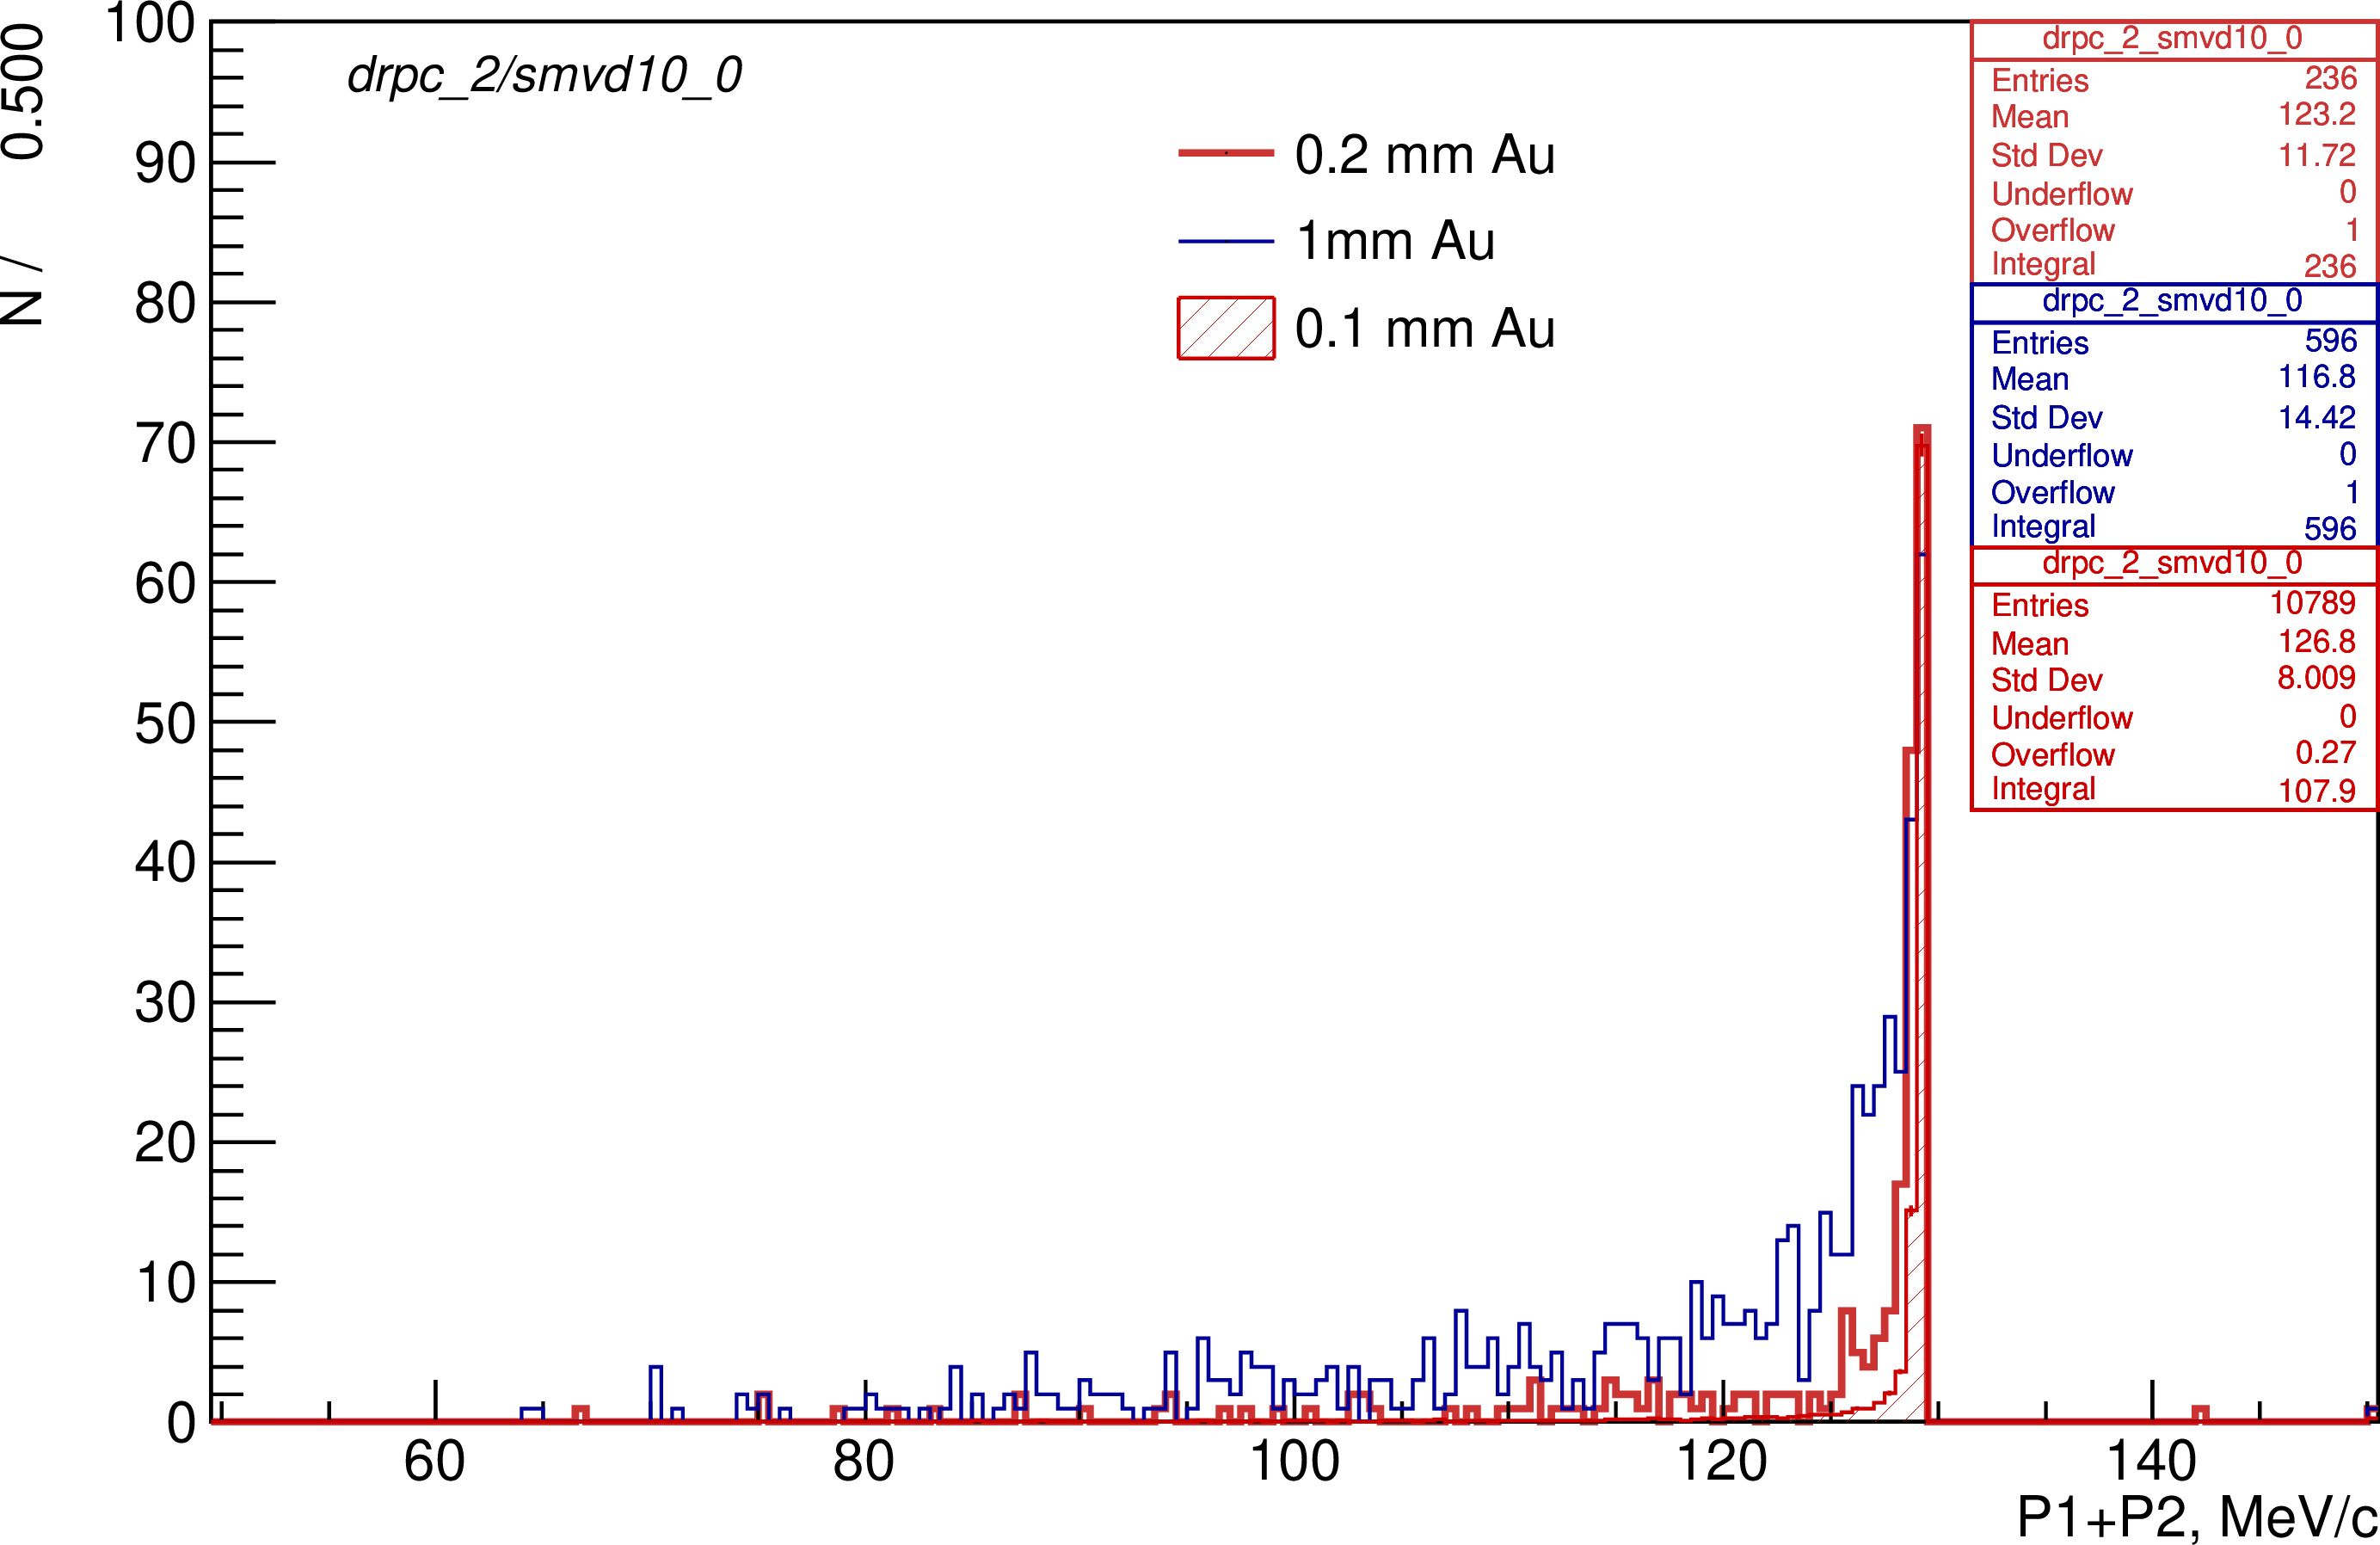
\includegraphics[width=0.54\textwidth]{pdf/figure_00010}
      % }
    };
    % \node [text width=8cm, scale=1.0] at (14.5,0.5) {$\mu_B$, expected background mean};
    % \node [text width=8cm, scale=1.0, rotate={90}] at (1.5,7.5) { $S_{D}$, ``discovery'' signal strength  };
  \end{tikzpicture}
  \caption{
    \label{figure:sum_mom_vd13}
    left: $E_\gamma^{VD13}$ for 1mm, 200 um, and 100-um thick Au converters at R=25 cm ; \\
    right: distributions of $E_\gamma^{VD10}$ for 1mm, 200 um, and 100-um thick Au converters at R=25 cm
  }
\end{figure}

The left plot in Figure~\ref{figure:sum_mom_vd13} illustrates that while the increasing
thickness of the converter improves the overall event yield of $\gamma \to e^+e^-$ events,
the thinnest considered converter foil produces more $\gamma \to e^+e^-$ events in the highest
energy bins than two other foils.

Comparison of the left and right plots in Figure~\ref{figure:sum_mom_vd13} shows the scale of energy
losses in the IPA and in the converter ring itself - significant fraction of energy losses comes
from the IPA.

\begin{figure}[H]
  \begin{tikzpicture}
    \node[anchor=south west,inner sep=0] at (0,0.) {
      % \node[shift={(0 cm,0.cm)},inner sep=0,rotate={90}] at (0,0) {}
      \makebox[\textwidth][c] {
        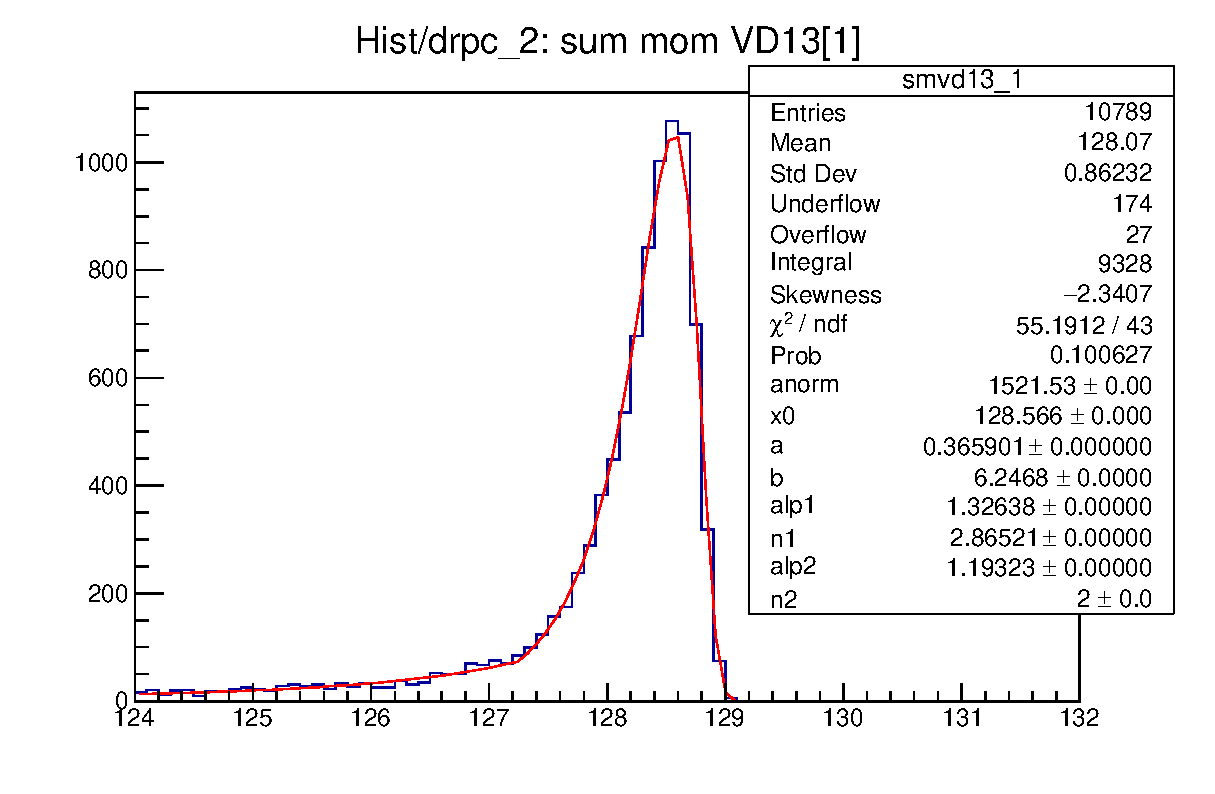
\includegraphics[width=0.9\textwidth]{pdf/figure_00083}
      }
    };
    % \node [text width=8cm, scale=1.0] at (14.5,0.5) {$\mu_B$, expected background mean};
    % \node [text width=8cm, scale=1.0, rotate={90}] at (1.5,7.5) { $S_{D}$, ``discovery'' signal strength  };
  \end{tikzpicture}
  \caption{
    \label{figure:00083}
    fit of the $E_\gamma^{VD13}$ distribution with the SU2020 resolution function defined by
    the Eq.\ref{eq:dio_mom_res}.
    The mean energy loss of two particles traveling from the converter to the tracker is about 0.8 MeV,
    the contribution of struggling to the energy resolution is $\sim 0.7$ MeV/c FWHM. \\
    The fit uncertainty on x0, parameter corresponding to the maximum of the fit function,
    is less than 1 keV.
  }
\end{figure}

Figure ~\ref{figure:00083} shows the distribution of $E_\gamma^{VD13}$
for 100 um converter with the binning of 100 keV/c. The distribution is fit
with the asymmetric resolution function introduced in the SU2020 paper \cite{MU2E_SU2020_PAPER}:

\begin{equation}
  \label{eq:dio_mom_res}
  R(x) =
 \begin{cases}
    A_1 \cdot (B_1-x)^{-N_1}                                 & x < -\alpha_1 \\
    A_0 \cdot \exp (a_0 \cdot (b_0 \cdot x - e^{b_0 \cdot x})) & -\alpha_1< x < \alpha_2 \\
    A_2 \cdot (B_2+x)^{-N_2}                                 &  x > \alpha_2
  \end{cases}.
\end{equation}
, where $x = p-p_0$, and $p_0$ is the position of the distribution maximum.
The most probable energy loss is about 800 keV/c, 
and the resolution function has the FWHM of about 700 keV/c.
These numbers are not very different from the corresponding numbers for conversion electrons.

The distribution of $E_\gamma^{VD10}$, the sum of the MC \eplus\ and \eminus\ momenta at VD10,
before the IPA, is shown in Figure ~\ref{figure:00086}. As the particles do not cross the
stopping target, this distribution reflects the impact on the energy resolution
of the converter itself.
%
Fluctuations of the energy losses in the 100 um gold converter result
in the FWHM of about 400 keV/c, small compared to the contribution of the IPA.
Interestingly, for a 100 keV/c binning, the highest energy bin is still
the most populated bin of the distribution.

\begin{figure}[H]
  \begin{tikzpicture}
    \node[anchor=south west,inner sep=0] at (0,0.) {
      % \node[shift={(0 cm,0.cm)},inner sep=0,rotate={90}] at (0,0) {}
      \makebox[\textwidth][c] {
        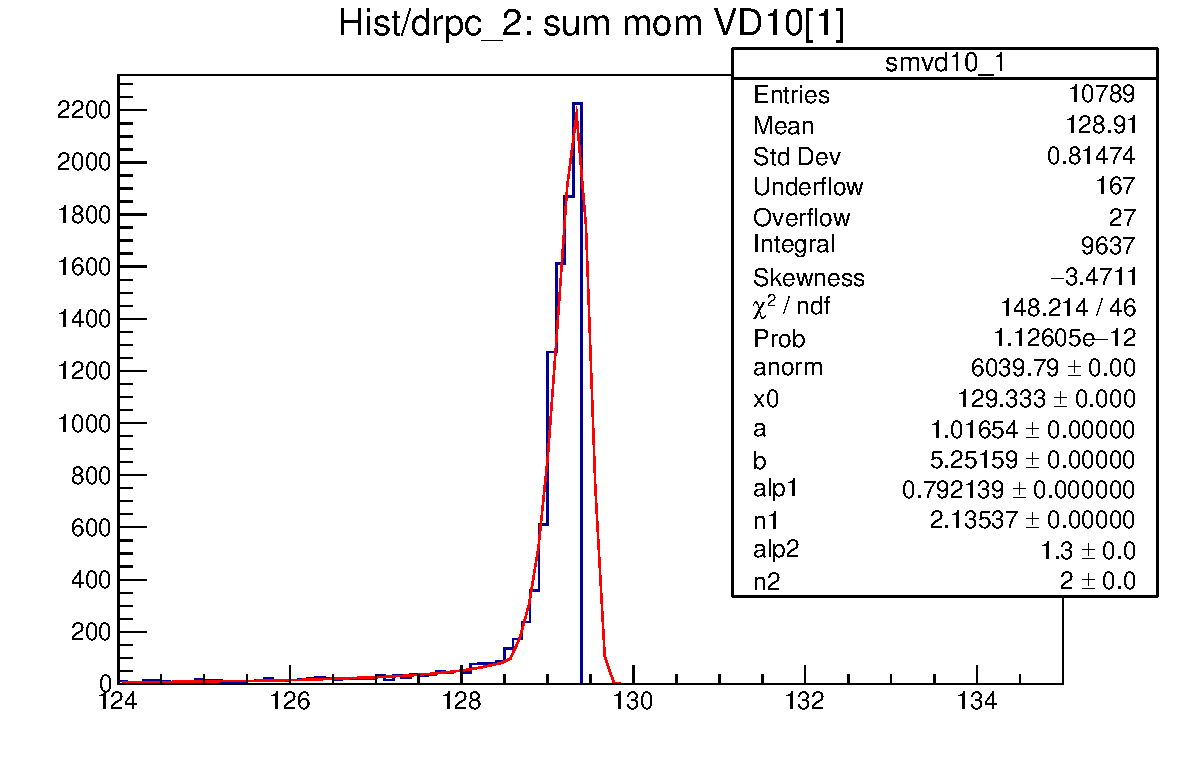
\includegraphics[width=0.9\textwidth]{pdf/figure_00086}
      }
    };
    % \node [text width=8cm, scale=1.0] at (14.5,0.5) {$\mu_B$, expected background mean};
    % \node [text width=8cm, scale=1.0, rotate={90}] at (1.5,7.5) { $S_{D}$, ``discovery'' signal strength  };
  \end{tikzpicture}
  \caption{
    \label{figure:00086}
    The distribution of $E_\gamma^{VD10}$, the sum of the MC \eplus\ and \eminus\ momenta at VD10.
    The distribution FWHM of about 400 keV/c, and the highest energy bin is the most populated
    bin of the distribution.
    The fit with the SU2020 resolution function is shown only as an illustration.
  }
\end{figure}

%%% Local Variables:
%%% mode: latex
%%% TeX-master: t
%%% End:
